\begin{figure}[t]
    \centering
    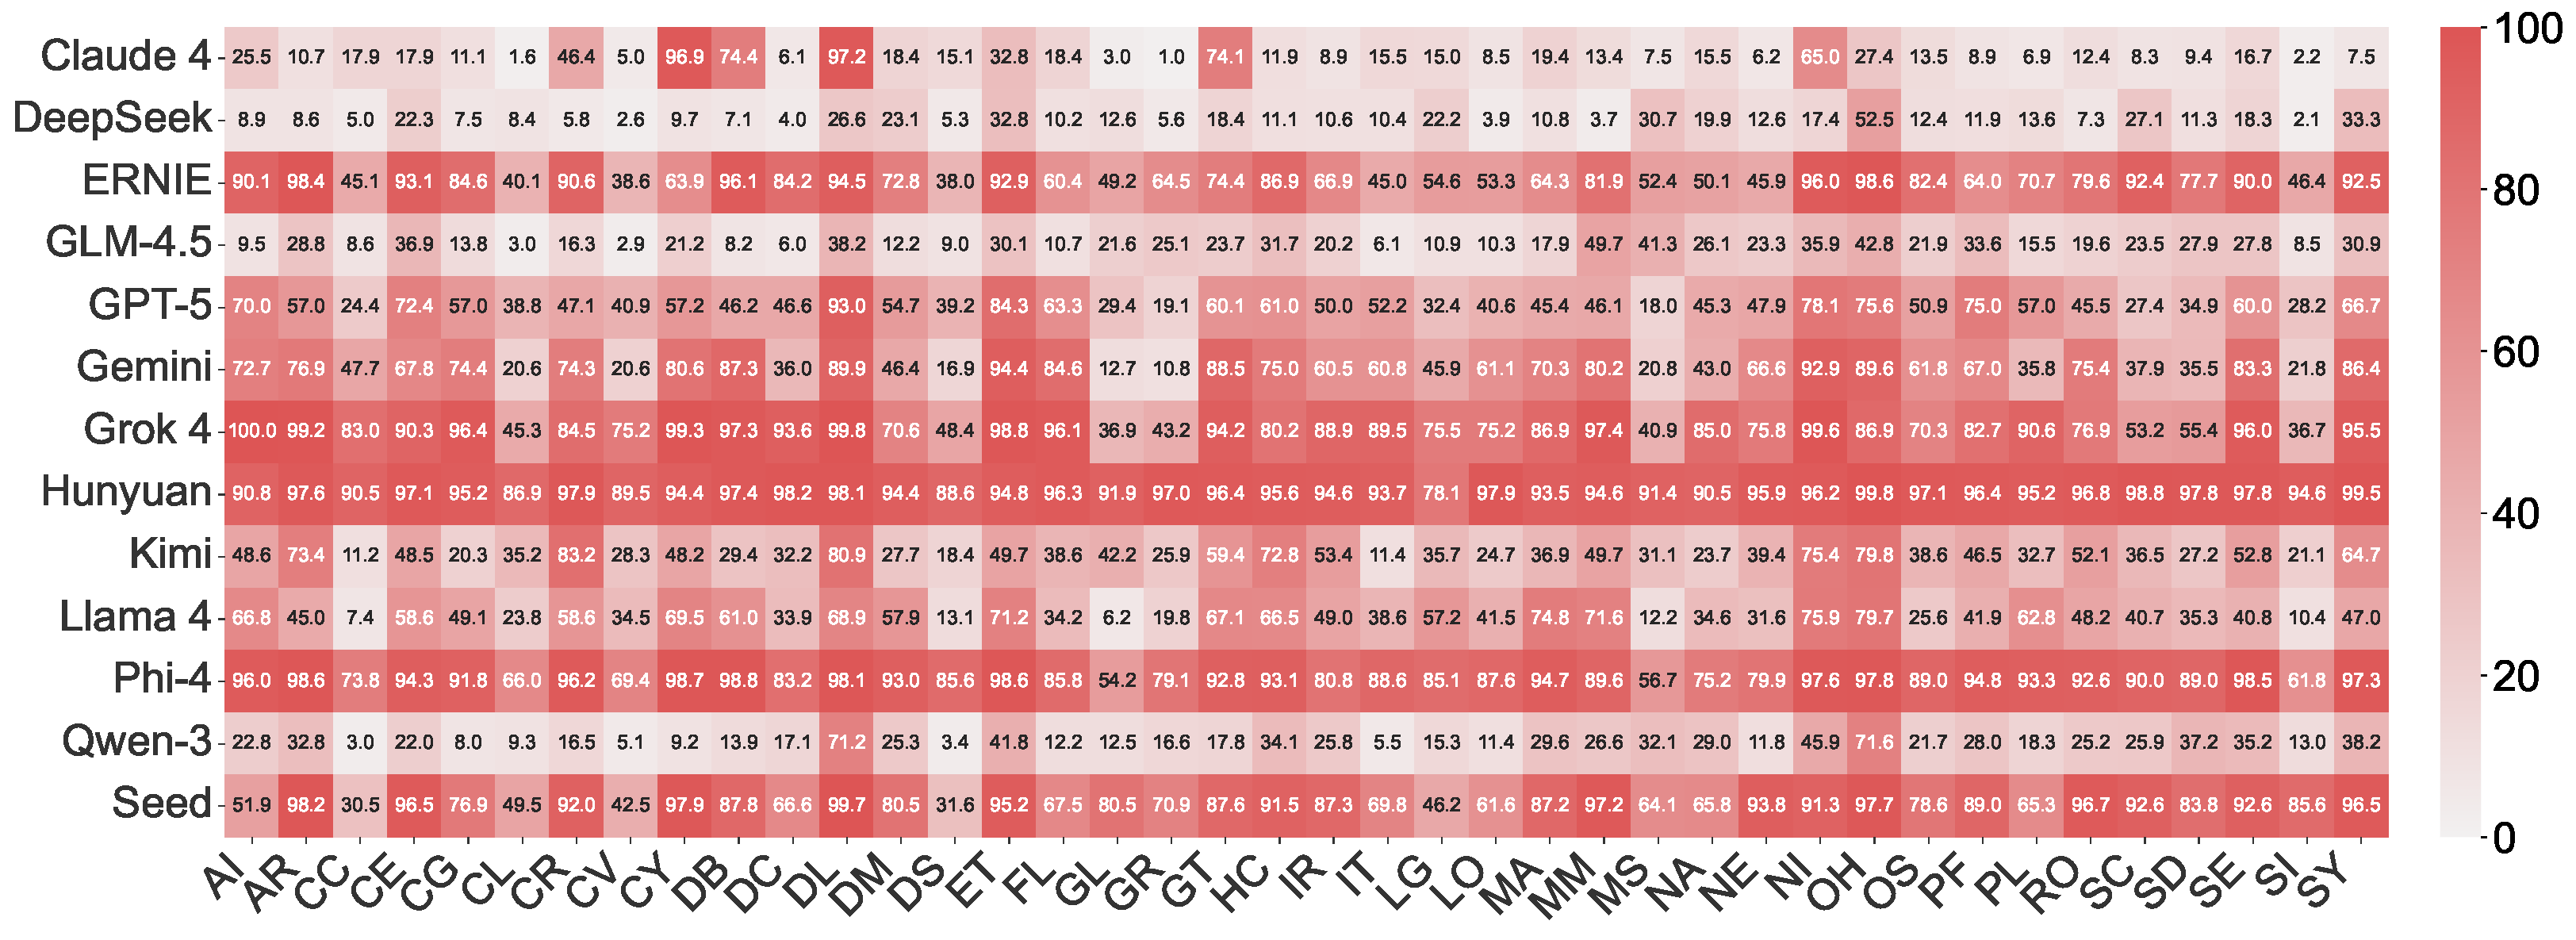
\includegraphics[width=\columnwidth]{Figures/Sec5_LLM/model_topic_heatmap.pdf}
    \vspace{-5.5mm}
    \caption{Model-domain hallucination rate heatmap. x-axis: models, y-axis: domains. Color represents the hallucination rate, the darker the color, the higher the hallucination rate.}
    \label{fig:model_topic_heatmap}
\end{figure}

% Input Correction and Specification
% The input contains a conceptual clarification: "The values in the figure represent the hallucination rate (Hallucination Rate) of generated citations; higher values (darker colors) indicate worse performance." The request is to provide a technical explanation in English and conduct a Case Study based on this logic.

% Technical Analysis of the Heatmap
% This heatmap visualizes the Hallucination Rate of various Large Language Models (LLMs) across multiple specialized domains. In this specific metric space, a higher numerical value (represented by darker purple) signifies a higher frequency of fabricated or incorrect citations, indicating lower factual reliability. Conversely, lower values (represented by yellow) indicate superior performance in citation accuracy.

% 1. Statistical Distribution and Domain Vulnerability
% High-Error Clusters (Dark Zones): Models such as Grok 4, Hunyuan, and Phi-4 exhibit widespread dark coloring, with scores frequently exceeding 80% or 90%. This indicates a systemic failure in maintaining factual grounding (Grounding) within these specific architectures or training datasets when generating references.

% Low-Error Clusters (Light Zones): Models like DeepSeek, GLM-4.5, and Qwen-3 demonstrate significantly lower hallucination rates (frequently < 20%). This suggests the integration of more robust Retrieval-Augmented Generation (RAG) mechanisms or higher-quality training data that prioritize source attribution accuracy.

% Case Study: Comparative Analysis of Citation Reliability
% To elucidate the implications of this data, two distinct cases are analyzed:

% Case A: Domain-Specific Failure in "AR" (Augmented Reality)
% Data Point: Grok 4 (97.0) vs. DeepSeek (8.3).

% Mechanism Analysis: In the AR domain, Grok 4 exhibits a near-total failure in citation veracity. This suggests that when queried for technical specifications or academic papers in AR, the model likely engages in Stochastic Parroting, generating plausible-sounding but non-existent bibliographic metadata (e.g., hallucinated DOIs or fake author-title pairings). In contrast, DeepSeek’s low score (8.3) indicates that its output is largely constrained by verified external knowledge or a more conservative decoding strategy that avoids speculative generation.

% Case B: Model Architecture Divergence in "DL" (Deep Learning)
% Data Point: GPT-5 (86.6) vs. Claude 4 (89.4) vs. Qwen-3 (42.5).

% Mechanism Analysis: Despite being frontier models, both GPT-5 and Claude 4 show high hallucination rates in the Deep Learning category. This phenomenon often occurs due to Knowledge Cutoff pressures or the over-reliance on internal parametric memory (Parametric Memory) for rapidly evolving technical fields. The models attempt to synthesize "perfect" citations that fit the context but do not exist in the physical world. Qwen-3, while still showing a moderate error rate (42.5), performs significantly better, potentially due to specialized fine-tuning on academic literature which reinforces the structural integrity of reference strings.

% Conclusion
% The data indicates that model scale does not inherently correlate with citation accuracy. Smaller or domain-optimized models (e.g., Qwen-3, DeepSeek) consistently outperform larger-parameter counterparts (e.g., Grok 4, GPT-5) in minimizing hallucinatory outputs. The high variance across the horizontal axis (X-axis) further confirms that certain technical domains (e.g., AI, CY, DL) are more prone to triggering the "hallucination mechanism" within the Transformer architecture's latent space.
